\documentclass[12pt,a4paper]{article}
\usepackage[utf8]{inputenc}
\usepackage[german]{babel}
\usepackage[T1]{fontenc}
\usepackage{amsmath}
\usepackage{amsfonts}
\usepackage{amssymb}
\usepackage{graphicx}
\usepackage{siunitx}
\usepackage{float}
\usepackage[left=2cm,right=2cm,top=2cm,bottom=2cm]{geometry}
\author{Gerald}

\begin{document}
\sisetup{separate-uncertainty = true}
	\setlength{\parindent}{0pt} 
	\begin{center}
		{\LARGE Versuchsprotokoll}\\
		\begin{large}
			zum Fortgeschrittenenpraktikum im Bachelorstudiengang Physik\\[0.4cm]
			an der RWTH Aachen\\
			II. Physikalisches Institut A\\[5.5cm]
			\Large\textbf{\textsl{Rastertunnelmikroskopie (STM)}}\\[5.5cm]
			\normalsize\textit{vorgelegt\\von}\\[0.4cm]
			\large{Moritz Berger (355244)\\Gerald Kolter (355005)}\\Gruppe 30\\[2cm]
			\large \textbf{Wintersemester 2017/18}
		\end{large}
	\end{center}
	\newpage
	
	\tableofcontents
	\newpage

\section{Versuchsziel}
Das Ziel des Versuchs besteht darin, mit einem Rastertunnelmikroskop bei der Vermessung einer Goldprobe die Auswirkung der Einstellungen auf das Messergebnis zu untersuchen. Mit einer Probe eines hochorientierten pyrolytischen Graphit (HOPG) wird der Abstand der Gitterebenen bestimmt und eine Kalibration in x- und y-Richtung durchgeführt.

\section{Aufbau}
Das verwendete Rastertunnelmikroskop besteht aus einem Halter für die Platin-Iridium-Spitze, der mit piezoelektrischen Kristallen in allen drei Raumrichtungen bewegt werden kann, und einem Probenhalter, der auf einem sogenannten Schrittmotorantrieb liegt. Dieser funktioniert ebenfalls mit einem piezoelektrischen Kristall und dient lediglich der Grobannäherung. Spitze und Probe sind über eine Spannungsquelle verbunden, wobei gleichzeitig der in diesem Kreis fließende Strom gemessen wird. Dieser Strom kommt bei kleinen Abständen zwischen Spitze und Probe durch den Tunneleffekt zustande. Die Abhängigkeit zwischen Strom und Abstand ist exponentiell und damit sehr stark.\\
Die Spitze wird mit den piezoelektrischen Kristallen über die Probe gerastert, wobei jede Linie in x-Richtung vorwärts und rückwärts abgefahren wird.\\
Eine Regelungselektronik steuert die z-Richtung der Spitze in Abhängigkeit des Tunnelstroms. Dabei gibt der sogenannte I-Gain an, wie schnell die Regelung auf kurze Pulse reagiert.

\section{Durchführung}
\subsection{Untersuchung der Mikroskopeigenschaften mit einer Goldprobe}

\begin{table}
\centering
\begin{tabular}{|c|c|}
\hline 
Bereichgröße & (75,23 nm)$^2$ \\ 
\hline 
Zeit pro Linie & 0,2 s \\
\hline 
Tunnelspannung & 450 mV \\ 
\hline 
Messpunkte pro Linie & 256 \\
\hline 
Sollwert Tunnelstrom & 1 nA \\
\hline 
\end{tabular} 
\caption{Einstellungen der Messparameter bei Vermessung der Goldprobe. Bei dieser Messreihe wurde der IGain zwischen 1000 und 11000 verändert.}
\label{tab:IGain_Einstellungen}
\end{table}

Für die Untersuchung der Empfindlichkeit der Einstellparameter wird auf der Goldprobe zunächst ein Bereich mit markanter Struktur gesucht. Dieser Bereich wird für vier verschiedene Werte für den I-Gain bei ansonsten gleichbleibenden Parametern vermessen. Diese Einstellungen sind in Tabelle \ref{tab:IGain_Einstellungen} eingetragen.\\
In einer zweiten Messreihe wird erneut ein Bereich mit markanter Struktur vermessen, wobei anstelle des I-Gain die Messzeit pro Zeile verändert wird. Für den I-Gain wurde hierbei der Wert, der sich in der ersten Messreihe als beste Annäherung des Idealwertes herausgestellt hat, verwendet (I-Gain = 3000). Alle anderen Parameter blieben unverändert.

\subsection{Untersuchung von HOPG}

\section{Ergebnisse}
\subsection{Untersuchung der Mikroskopeigenschaften mit einer Goldprobe}

\begin{figure}
\centering
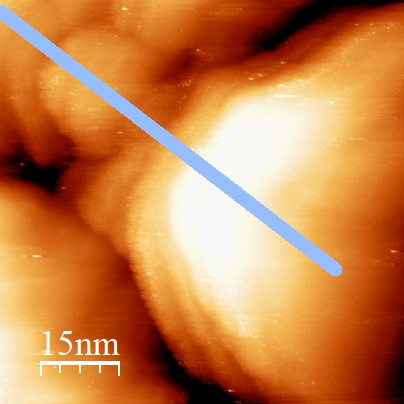
\includegraphics[scale=0.8]{Bilder/3000_IGain_vor.jpg}
\caption{Bild der z-Komponente bei Vermessung der Goldprobe mit einem I-Gain von 3000 in der Vorwärtsrichtung. Der Balken quer im Bild verbildlicht die Stelle, aus der das Höhenprofil entnommen wurde.}
\label{fig:Gold_IGain_Beispiel}
\end{figure}

\begin{figure}
\centering
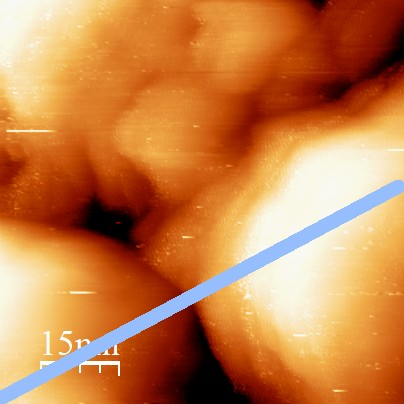
\includegraphics[scale=0.8]{Bilder/0_1_Zeit_vor.jpg}
\caption{Bild der z-Komponente bei Vermessung der Goldprobe bei einer Messzeit von 0,1s pro Linie in der Vorwärtsrichtung. Der Balken quer im Bild verbildlicht die Stelle, aus der das Höhenprofil entnommen wurde.}
\label{fig:Gold_Zeit_Beispiel}
\end{figure}

Abbildung \ref{fig:Gold_IGain_Beispiel} zeigt beispielhaft das Bild der z-Komponente nach Bearbeitung für eine Messung aus der Messreihe mit verändertem I-Gain. Der Balken quer im Bild zeigt, wo das im Folgenden untersuchte Höhenprofil entnommen wurde. In den Bildern aus den Ergebnissen der Messreihe wurde das Höhenprofil exakt gleich entnommen (Profillinie kopiert), sodass die Vergleichbarkeit der Profile gegeben ist.\\
Bei der Aufnahme der Messreihe mit veränderter Zeit wurde ein anderer Bereich verwendet. Daher ist die Profillinie aus einem anderen Bildbereich entnommen, wie in Abbildung \ref{fig:Gold_Zeit_Beispiel} dargestellt ist.\\
Bei der Entnahme des Höhenprofils wird für jeden Wert der Mittelwert mehrerer Punkte bestimmt.

\subsubsection{Bestimmung der Flankensteigung}
Zur Bestimmung der Flankensteigung werden die Punkte, die diese Flanke begrenzen, abgelesen.
Die Flankensteigung berechnet sich dann zu:

\begin{equation*}
a = \dfrac{Z_2 - Z_1}{X_2 - X_1}
\end{equation*}

Als Fehler auf die Werte wird der Ablesefehler

\begin{equation*}
\sigma = \dfrac{\SI{0.1}{nm}}{\sqrt{12}}
\end{equation*}

auf jeden abgelesenen Wert angenommen, sodass sich der Fehler auf die Steigung fortpflanzt zu:

\begin{equation*}
\sigma _a = \sqrt{2 \cdot \left( \dfrac{\sigma}{X_2 - X_1} \right) ^2 + 2 \cdot \left( \sigma \cdot  \dfrac{Z_2 - Z_1}{(X_2 - X_1)^2} \right) ^2}
\end{equation*}


\subsubsection{Untersuchung der Auswirkungen des I-Gain}

\begin{table}
\centering
\begin{tabular}{|c|c|c|}
\hline 
IGain & Peakpositionen in Vorwärtsrichtung [nm] & Peakpositionen in Rückwärtsrichtung [nm] \\ 
\hline 
1000 & (23.4, 0.0), (50.1, 3.4) & (27.5, 0.0), (44.7, 2.9) \\
\hline 
3000 & (36.5, 0.0), (48.2, 2.4) & (32.7, 0.0), (44.7, 2.6) \\ 
\hline 
8000 & (31.5, 0.0), (45.9, 4.4) & (28.0, 0.1), (44.0, 3.5) \\
\hline 
11000 & (30.8, 0.0), (48.6, 8.3) & (30.8, 0.0), (41.4, 9.4) \\
\hline 
\end{tabular} 
\caption{Abgelesene Werte für die Begrenzungen der Flanken in der Messreihe zur Variation des I-Gain.}
\label{tab:Peaks_IGain}
\end{table}

\begin{figure}
\centering
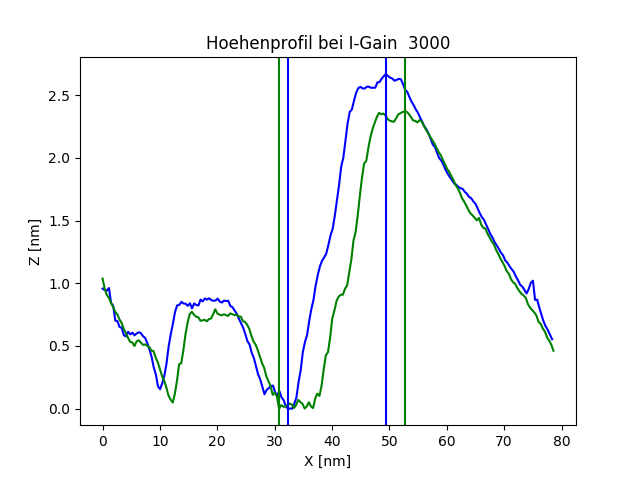
\includegraphics[scale=0.8]{Bilder/Profil_IGain_3000_Peakbestimmung.png}
\caption{Höhenprofil bei einem I-Gain von 3000. Die roten Linien markieren die abgelesenen Flanken.}
\label{fig:Gold_IGain_Flankensteigung}
\end{figure}

Tabelle \ref{tab:Peaks_IGain} zeigt alle abgelesenen Werte für diese Punkte in der Messreihe zum I-Gain. Abbildung \ref{fig:Gold_IGain_Flankensteigung} zeigt beispielhaft die gemessenen Höhenprofile und die abgelesenen Flanken bei einem IGain von 3000. 

\begin{table}
\centering
\begin{tabular}{|c|c|c|c|}
\hline 
IGain & $a_{vor}$ & $a_{rueck}$ & $\dfrac{|a_{vor} - a_{rueck}|}{\sqrt{\sigma _{a_{vor}}^2 + \sigma _{a_{rueck}}^2}}$ \\ 
\hline 
1000 & 0,1273 $\pm$ 0,0015 & 0,1686 $\pm$ 0,0024 & 14,44 \\
\hline 
3000 & 0,2051 $\pm$ 0,0036 & 0,2167 $\pm$ 0,0035 & 2,32 \\ 
\hline 
8000 & 0,3056 $\pm$ 0,0030 & 0,2125 $\pm$ 0,0026 & 23,57 \\
\hline 
11000 & 0,4663 $\pm$ 0,0025 & 0,8868 $\pm$ 0,0051 & 73,31 \\
\hline 
\end{tabular} 
\caption{Berechnete Flankensteigungen und die Abweichung zwischen der Steigung aus der Messung in Vorwärts- und der in Rückwärtsrichtung für die Messreihe mit variiertem I-Gain.}
\label{tab:Steigungen_IGain}
\end{table}

Tabelle \ref{tab:Steigungen_IGain} zeigt die Ergebnisse für die Flankensteigungen. Die Abweichungen zwischen den Steigungen aus der Messung in Vorwärts- und der in Rückwärtsrichtung zeigen, dass bei einer Messzeit von \SI{200}{ms} ein I-Gain von 3000 die besten Ergebnisse liefert.

\subsubsection{Untersuchung der Auswirkungen der Zeit}

\begin{table}
\centering
\begin{tabular}{|c|c|c|}
\hline 
Zeit [ms] & Peakpositionen in Vorwärtsrichtung [nm] & Peakpositionen in Rückwärtsrichtung [nm] \\ 
\hline 
52 & (33.0, 0.0), (51.1, 3.5) & (28.5, 0.0), (45.3, 3.4) \\
\hline 
80 & (22.2, 0.0), (54.8, 3.6) & (20.2, 0.0), (46.0, 3.5) \\ 
\hline 
100 & (38.6, 0.0), (54.2, 3.4) & (35.2, 0.0), (50.9, 3.7) \\
\hline 
200 & (18.7, 0.0), (53.8, 4.2) & (15.5, 0.0), (48.4, 4.2) \\
\hline 
400 & (36.5, 0.0), (53.1, 3.1) & (33.6, 0.0), (50.7, 3.5) \\
\hline 
600 & (27.6, 0.0), (52.7, 3.4) & (24.6, 0.0), (48.6, 3.3) \\
\hline 
2000 & (43.6, 0.0), (62.8, 3.1) & (38.8, 0.0), (57.0, 2.7) \\
\hline 
\end{tabular} 
\caption{Abgelesene Werte für die Begrenzungen der Flanken in der Messreihe zur Variation der Zeit.}
\label{tab:Peaks_Zeit}
\end{table}

\begin{figure}
\centering
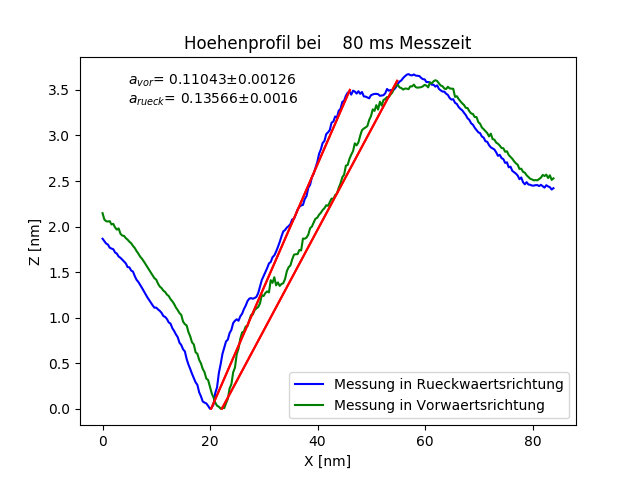
\includegraphics[scale=0.8]{Bilder/Profil_Zeit_80_Peakbestimmung.png}
\caption{Höhenprofil bei einer Messzeit von \SI{80}{ms}. Die roten Linien markieren die abgelesenen Flanken.}
\label{fig:Gold_Zeit_Flankensteigung}
\end{figure}

Tabelle \ref{tab:Peaks_Zeit} zeigt alle abgelesenen Werte für diese Punkte in der Messreihe zum I-Gain. Abbildung \ref{fig:Gold_Zeit_Flankensteigung} zeigt beispielhaft die gemessenen Höhenprofile und die abgelesenen Flanken bei einer Messzeit von \SI{80}{ms}.

\begin{table}
\centering
\begin{tabular}{|c|c|c|c|}
\hline 
Zeit [ms] & $a_{vor}$ & $a_{rueck}$ & $\dfrac{|a_{vor} - a_{rueck}|}{\sqrt{\sigma _{a_{vor}}^2 + \sigma _{a_{rueck}}^2}}$ \\ 
\hline 
52 & 0,1934 $\pm$ 0,0023 & 0,2024 $\pm$ 0,0025 & 2,67 \\
\hline 
80 & 0,1104 $\pm$ 0,0013 & 0,1357 $\pm$ 0,0016 & 12,40 \\ 
\hline 
100 & 0,2179 $\pm$ 0,0027 & 0,2357 $\pm$ 0,0027 & 4,68 \\
\hline 
200 & 0,1197 $\pm$ 0,0012 & 0,1277 $\pm$ 0,0013 & 4,67 \\
\hline 
400 & 0,1867 $\pm$ 0,0025 & 0,2047 $\pm$ 0,0024 & 5,13 \\
\hline 
600 & 0,1355 $\pm$ 0,0016 & 0,1375 $\pm$ 0,0017 & 0,86 \\
\hline 
2000 & 0,1615 $\pm$ 0,0022 & 0,1484 $\pm$ 0,0023 & 4,19 \\
\hline 
\end{tabular} 
\caption{Berechnete Flankensteigungen und die Abweichung zwischen der Steigung aus der Messung in Vorwärts- und der in Rückwärtsrichtung für die Messreihe mit variierter Zeit pro Zeile.}
\label{tab:Steigungen_Zeit}
\end{table}

Tabelle \ref{tab:Steigungen_Zeit} zeigt die Ergebnisse für die Flankensteigungen. Die Abweichungen zwischen den Steigungen aus der Messung in Vorwärts- und der in Rückwärtsrichtung zeigen, dass bei einem I-Gain von 3000 eine Messzeit pro Zeile von \SI{600}{ms} die besten Ergebnisse liefert.

\subsubsection{Zusammenfassung}
Mit steigendem I-Gain werden die gemessenen Flankensteigungen größer. Dabei liegt der ideale I-Gain in einem mittleren Bereich, wo die gemessenen Flankensteigungen aus der Vorwärts- und der Rückwärtsrichtung nahe zusammenrücken. \\
Bei der zweiten Messreihe mit Variation der Messzeit pro Zeile hat sich herausgestellt, dass bei einem I-Gain von 3000 und einer Messzeit von \SI{600}{ms} die Flankensteigungen aus der Vorwärts- und der Rückwärtsrichtung innerhalb einer Standardabweichung übereinstimmen.

\subsection{Untersuchung von HOPG}

\section{Fazit}

\section{Anhang}


\end{document}